\section{【原理】进程的属性与特征解析}\label{ux539fux7406ux8fdbux7a0bux7684ux5c5eux6027ux4e0eux7279ux5f81ux89e3ux6790}

为了让多个程序能够使用CPU执行任务,我们需要设计进程控制块,需要进一步管理进程。但到底如何设计进程控制块,如何管理进程?如果我们对进程的属性和特征了解不够,则无法有效地设计进程控制块和实现进程管理。

再一次回到进程的定义:一个具有一定独立功能的程序在一个数据集合上的一次动态执行过程。这里有四个关键词:程序、数据集合、执行、动态执行过程。从CPU的角度来看,所谓程序就是一段特定的指令机器码序列而已。CPU会一条一条地取出在内存中程序的指令并按照指令的含义执行各种功能。所谓数据集合就是使用的内存,所谓执行就是让CPU工作。那么这个数据集合和执行其实体现了进程对资源的占用。动态执行过程体现了程序执行的不同``生命''阶段:诞生、工作、休息/等待、死亡。如果这一段指令执行完毕,也就意味着进程结束了。从开始执行到执行结束是一个进程的全过程。那么操作系统需要管理进程的什么?如果计算机系统中只有一个进程,那操作系统的工作就简单了。其实就是管理进程执行的指令,进程占用的资源,进程执行的状态。这可归结为对一个进程内的管理工作。但实际上在计算机系统的内存中,可以放很多程序,这也就意味着操作系统需要管理多个进程,那么,还需要做有关进程间的其他管理工作包括:进程调度、进程间的数据共享、进程间执行的同步互斥关系(lab5涉及)等。下面逐一进行解析。

\subsection{指令执行安全管理}\label{ux6307ux4ee4ux6267ux884cux5b89ux5168ux7ba1ux7406}

CPU的指令有一般指令和特权指令之分,那么由不包含特权指令的一般指令集合组成了用户程序,而由特权指令加上一般指令形成的核心软件就是操作系统了。CPU在执行时可处于不同的特权模式:用户态模式和核心态模式,在用户态模式只能执行一般指令,在核心态模式除了可以执行一般指令外,还可以执行特权指令。如果这里的程序是指的一般应用程序或用户程序,不是操作系统,那么我们把在CPU处于用户态特权模式下的应用程序的执行过程称为用户进程。如果这里的程序指的是操作系统,那么我们把在CPU处于核心态特权模式下的操作系统的执行过程称为内核进程。回想lab1和lab2中内容,物理内存在操作系统的内存管理下也有类型,可以分为用户态内存和核心态内存,这两种内存形成了CPU可能访问的所有内存空间。内核进程可以干任何事情,所以对于各种内存,各种指令,它都能访问和执行。用户进程和内核进程对内存和指令的权限如下所示:

\begin{figure}[htbp]
\centering
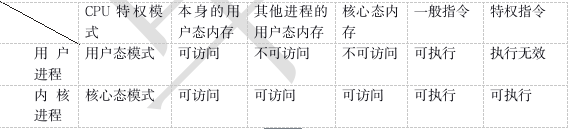
\includegraphics{figures/0.png}
\caption{0}
\end{figure}

用户进程本身要完成的工作细节由一条一条指令具体体现。对于一般指令完成``合法''的功能,操作系统不用管理。操作系统要管理的是用户进程的``非法''指令。简单地说,``非法''指令包括:特权指令、引起异常的一般指令(比如除零操作)和访问不属于它的内存空间。

而且操作系统会在用户进程执行前,设置一个用户进程执行的用户态环境,即如果程序的指令流一开始执行,操作系统就让CPU处于用户态特权模式。而且还要分配一定的物理空间,建立页表,给进程一个用户态虚拟内存空间,这样一个用户态进程就可以在这个限定的虚拟内存空间中正常执行一般指令了。一旦用户进程执行了``非法''指令,则CPU会产生异常,CPU使用权将转到操作系统中,从而让操作系统能够对执行``非法''指令的用户进程进行管理,比如让进程退出、给进程分配更大的内存空间等。这样操作系统能够确保用户进程在执行过程中无法破坏在内存中的其他用户进程和操作系统本身。

\subsection{资源管理}\label{ux8d44ux6e90ux7ba1ux7406}

在计算机系统中,进程会占用内存和CPU,这都是有限的资源,如果不进行合理的管理,资源会耗尽或无法高效公平地使用,从而会导致计算机系统中的多个进程执行效率很低,甚至由于资源不够而无法正常执行。

对于用户态进程而言,操作系统是它的``上帝'',操作系统给了用户态进程可以运行所需的资源,最基本的资源就是内存和CPU。在lab2中涉及的内存管理方法和机制可直接应用到进程的内存资源管理中来。在有多个进程存在的情况下,对于CPU这种资源,则需要通过进程调度来合理选择一个进程,并进一步通过进程分派和进程切换让不同的进程分时复用CPU,执行各自的工作。进程调度的核心是各种进程调度算法,而调度算法的评价指标是高效、合理、公平、系统吞吐量大、响应时间短等。另外,对于无法剥夺的共享资源,如果资源管理不当,多个进程会出现死锁或饥饿现象

\subsection{状态管理}\label{ux72b6ux6001ux7ba1ux7406}

用户进程有不同的状态(也可理解为``生命''的不同阶段),当操作系统把程序的放到内存中后,这个进程就``诞生''了,不过还没有开始执行,但已经消耗了内存资源,处于``创建''状态;当进程准备好各种资源,就等能够使用CPU时,进程处于``就绪''状态;当进程终于占用CPU,程序的指令被CPU一条一条执行的时候,这个进程就进入了``工作''状态,也称``运行''状态,这时除了进一步占用内存资源外,还占用了CPU资源;当这个进程等待某个资源而无法继续执行时,进程可放弃CPU使用,即释放CPU资源,进入``等待''状态;当程序指令执行完毕,进程进入了``死亡''状态。

这些状态的转换时机需要操作系统管理起来,而且进程的创建和清除等工作必须由操作系统提供,而且从``运行''态与``就绪''态/``等待''态之间的转换,涉及到保存和恢复进程的``执行现场'',也成为进程上下文,这是确保进程即使``断断续续''地执行,也能正确完成工作的必要保证。

\subsection{系统调用}\label{ux7cfbux7edfux8c03ux7528}

操作系统把用户进程现在在用户态特权模式下执行,这使得用户进程无法完成各种重要的工作,比如获取内存、访问硬盘内容等。为了解决这个问题,用户进程可通过执行系统调用来通知操作系统帮助它来完成这些需要在特权态下才能执行的重要工作。执行系统调用会使得CPU从用户态特权模式切换到核心态特权模式,在用户进程的用户态执行现场(用户态进程运行上下文)也需要保存在操作系统中,当操作系统完成用户进程请求的工作后,还需根据保存的用户态执行现场恢复用户进程的正常执行。

\subsection{进程与线程}\label{ux8fdbux7a0bux4e0eux7ebfux7a0b}

一个进程拥有一个存放程序和数据的的虚拟地址空间以及其他资源。一个进程基于程序的指令流执行,其执行过程可能与其它进程的执行过程交替进行。因此,一个具有执行状态(运行态、就绪态等)的进程是一个被操作系统调度并分派的单位。在大多数操作系统中,这两个特点是进程的主要本质特征。但这两个特征相对独立,操作系统可以把这两个特征分别进行管理。

这样可以把拥有资源所有权的单位通常仍称作进程,对资源的管理成为进程管理;把指令执行流的单位称为线程,对线程的管理就是线程调度和线程分派。对属于同一进程的所有线程而言,这些线程共享进程的虚拟地址空间和其他资源,但每个线程都有一个独立的栈,还有独立的线程运行上下文用于包含表示线程执行现场的寄存器值等信息。

在多线程环境中,进程被定义成资源分配与保护的单位,与进程相关联的信息主要有存放进程映像的虚拟地址空间等。在一个进程中,可能有一个或多个线程,每个线程有线程执行状态(运行、就绪、死亡等),保存上次运行时的线程上下文、线程的执行栈等。考虑到CPU有不同的特权模式,参照进程的分类,线程又可进一步细化为用户线程和内核线程。

到目前为止,我们就可以明确用户进程、核心进程、用户线程、核心线程的区别了。从本质上看,线程就是一个特殊的不用拥有资源的轻量级进程,在ucore的调度和执行管理中,并没有区分线程和进程。且由于ucore内核中的所有内核进程共享一个内核地址空间和其他资源,所以这些内核进程都是内核线程。理解了进程或线程的上述属性和特征,我们就可以进行进程/线程管理的设计与实现了。但是为了叙述上的简便,在分析proj12(proj12实现了用户线程)以前,以下用户态的进程/线程统称为用户进程,而内核进程/线程则统称为内核线程。
